\section{Part Two: Implementing the Experts}
\subsection{Task 1: Forward and backward implementation}
The NumPy module implements the expert MLPs, selected-expert gates, residual addition, and prediction head specified in the handout~\citep{handout}. Samples are stored in rows, while weight arrays retain the prescribed column-vector convention. Expert computations are batched using \texttt{einsum}. Unselected router logits are masked before Softmax, and the supplied mask is retained during finite-difference checks. Prediction log-probabilities are computed using a shifted log-sum-exp expression for numerical stability.

Backpropagation uses NumPy only, with no automatic differentiation. The mean-loss scaling is applied once at the prediction logits. The input gradient accumulates the expert, router, and direct residual paths; the ReLU derivative at zero is set to zero. The two-expert numerical case gives loss $1.0986122886681098$, and the supplied three-expert Top-2 case gives loss $1.184281870559786$.

\subsection{Task 2: Central-difference verification}
The official checker uses float64, perturbation $\epsilon=10^{-6}$, and a fixed selection mask away from routing ties and ReLU kinks. Table~\ref{tab:numpy-gradients} reports the maximum normalized error for every parameter family and the input, using the normalization in the handout. All errors are below the required $10^{-5}$ threshold.
\begin{table}[ht]
\centering
\small
\caption{Maximum normalized central-difference errors.}
\label{tab:numpy-gradients}
\begin{tabular}{lrr}
\toprule
Quantity & Two-expert example & Three-expert Top-2 \\
\midrule
$W_1$ & 1.404e-11 & 1.370e-10 \\
$b_1$ & 1.075e-10 & 1.234e-10 \\
$W_2$ & 4.084e-11 & 1.173e-10 \\
$b_2$ & 9.348e-11 & 1.000e-10 \\
$G$ & 6.077e-11 & 8.208e-11 \\
$C$ & 4.270e-11 & 1.137e-10 \\
$b_c$ & 6.443e-11 & 1.600e-10 \\
$x$ & 4.142e-11 & 1.083e-10 \\
\bottomrule
\end{tabular}
\end{table}


The supplied faulty variant explicitly subtracts the direct residual contribution from the otherwise complete input gradient. It therefore omits the identity path from the input to the residual sum. Its normalized input error rises to $0.133333$ in the two-expert case and $0.279717$ in the sparse case. This distinguishes an incorrect shared-input gradient from the parameter gradients, which can still be correct when an input path is omitted.

\subsection{Task 3: Fixed-batch training}
Training uses the supplied 128 examples and initialization, fixed context features, 400 full-batch SGD updates, and learning rate $0.2$. No hyperparameter search was performed. Training cross-entropy decreases from $5.593877$ to $1.870696$ (Figure~\ref{fig:numpy-loss}). Table~\ref{tab:numpy-predictions} shows the three examples selected by the provided runner. Two are incorrect despite the loss reduction; this is a training demonstration, not evidence of generalization.
\begin{figure}[ht]
\centering
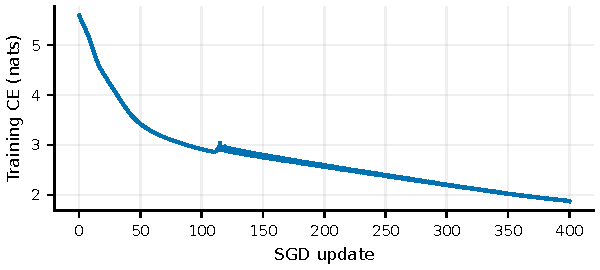
\includegraphics[width=.72\linewidth]{numpy_loss.pdf}
\caption{Mean training cross-entropy for the provided NumPy batch. The curve includes the initial loss and the loss after each of 400 SGD updates.}
\label{fig:numpy-loss}
\end{figure}
\begin{table}[ht]
\centering
\small
\caption{Three predictions after 400 NumPy SGD updates. Parentheses contain byte values.}
\label{tab:numpy-predictions}
\begin{tabular}{lll}
\toprule
Four-byte context & Target & Prediction \\
\midrule
\texttt{tle'} & s (115) & space (32) \\
\texttt{est=} & a (97) & e (101) \\
\texttt{u\textvisiblespace{}as} & space (32) & space (32) \\
\bottomrule
\end{tabular}
\end{table}

\FloatBarrier

